\chapter{航天器姿态运动学}
\thispagestyle{empty}

\section{航天器常用坐标系}
\subsection{基本概念}
\vspace*{-1em}

\defination[天体坐标系基本概念]
{
	\dy[天球]{TQ}\quad 指一个以地球质心$M$为中心,半径$r$为任意长的一个假想的球体 。其目的是将天体沿观测者视线投影到球面上,以便于研究天体及其相互关系。\\
	\hspace*{2.2em}\dy[黄道平面]{HDPM}\quad 由于地球绕太阳公公转而产生的,即地球公转轨道在天球上的反映称为黄道。它和赤道面相交于春分点和秋分点。\\
	\hspace*{2.2em}\dy[春分点]{CFD}\quad 指太阳从难向北在黄赤道上的交点。
}

\begin{figure}[!htb]
	\begin{minipage}{0.45\linewidth}
		\centering
		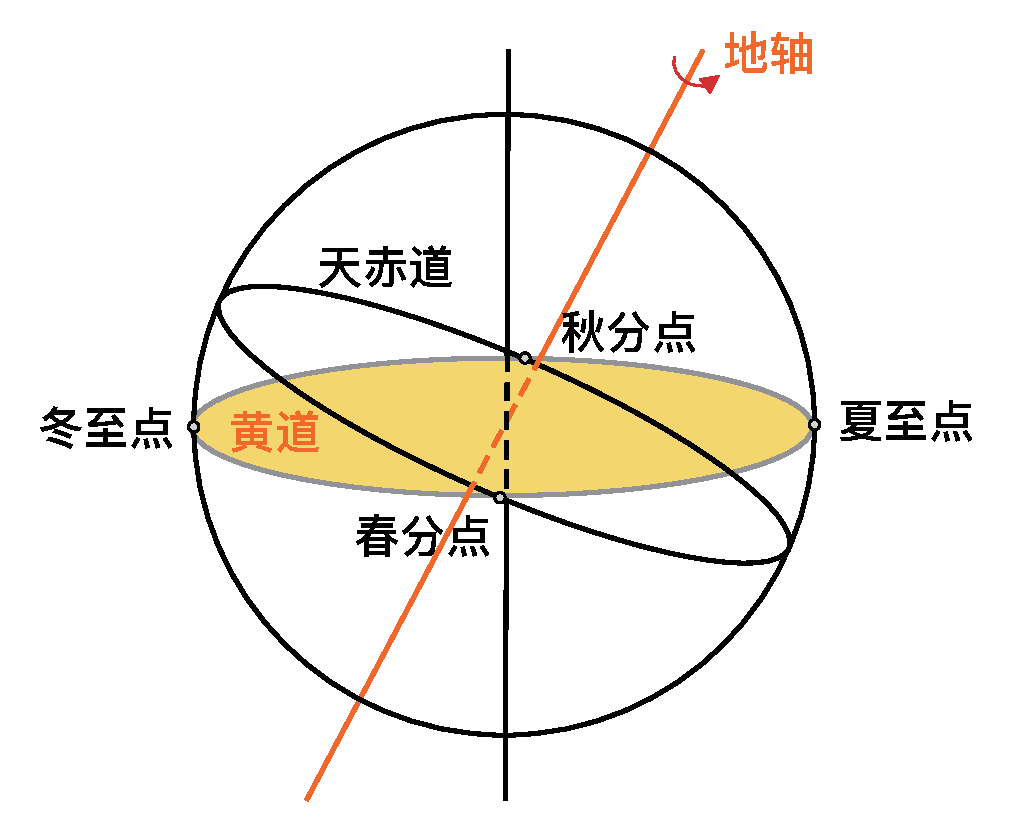
\includegraphics[width=\linewidth]{pic/基本概念}
		\caption{天球坐标系的基本概念}
		\label{基本概念}
	\end{minipage}
	\begin{minipage}{0.55\linewidth}
		\centering
		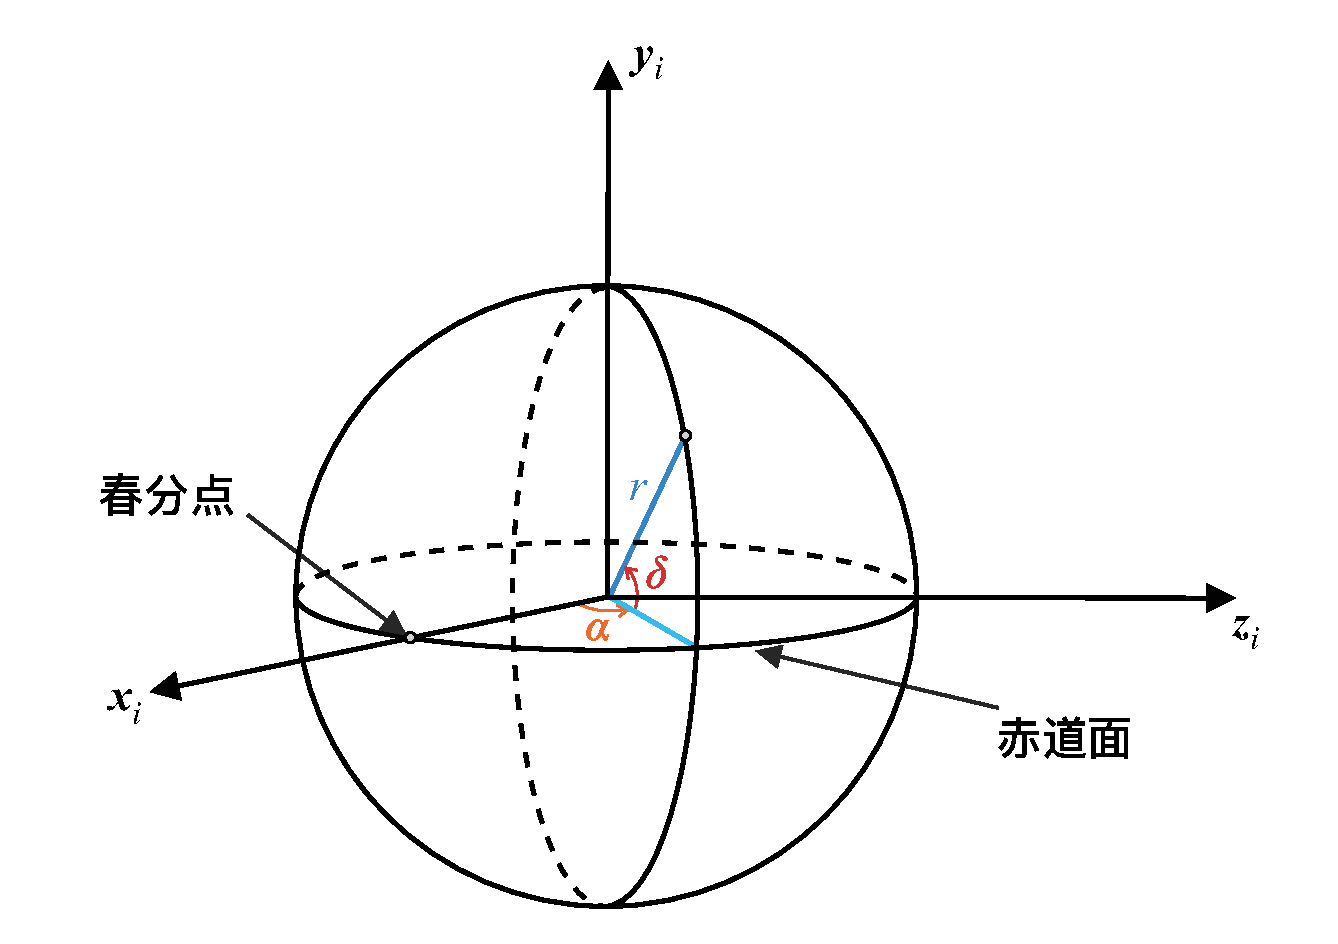
\includegraphics[width=\linewidth]{pic/地惯}
		\vspace*{-2.9em}
		\caption{地心赤道惯性坐标系}
		\label{地惯}
	\end{minipage}
\end{figure}


\subsection{地心赤道惯性坐标系}
\vspace*{-1em}

\defination[地心赤道惯性坐标系]
{
	如图 \ref{地惯} 所示,\dy[地心第一赤道坐标系]{DXDYCDZBX},简称为\dy[惯性坐标系]{GXZBX}。$X$轴在地球赤道平面内,指向赤道平面与黄道平面的相交线交点(春分点)。$Z$轴垂直于赤道平面,与地球自转角速度矢量方向一致。J2000的地心平赤道、平春分点的地心赤道坐标系。
}


\subsection{地心赤道旋转坐标系}
\vspace*{-1em}

\defination[地心赤道坐标系]
{
	如图 \ref{地心旋转} 所示,\dy[地心赤道旋转坐标系]{DXCDXZZBX},也叫\dy[地心第四赤道坐标系]{DXDSCDZBX}。$X$轴在赤道平面内,指向\dy[格林威治子午线]{GLNZZWX},$Z$轴垂直于赤道平面,与地球自转角速度矢量方向一致。$\lambda$是地理经度,从格林威治子午线向东度量,$\phi$是地心纬度。
}

\begin{figure}[!htb]
	\begin{minipage}{0.485\linewidth}
		\centering
		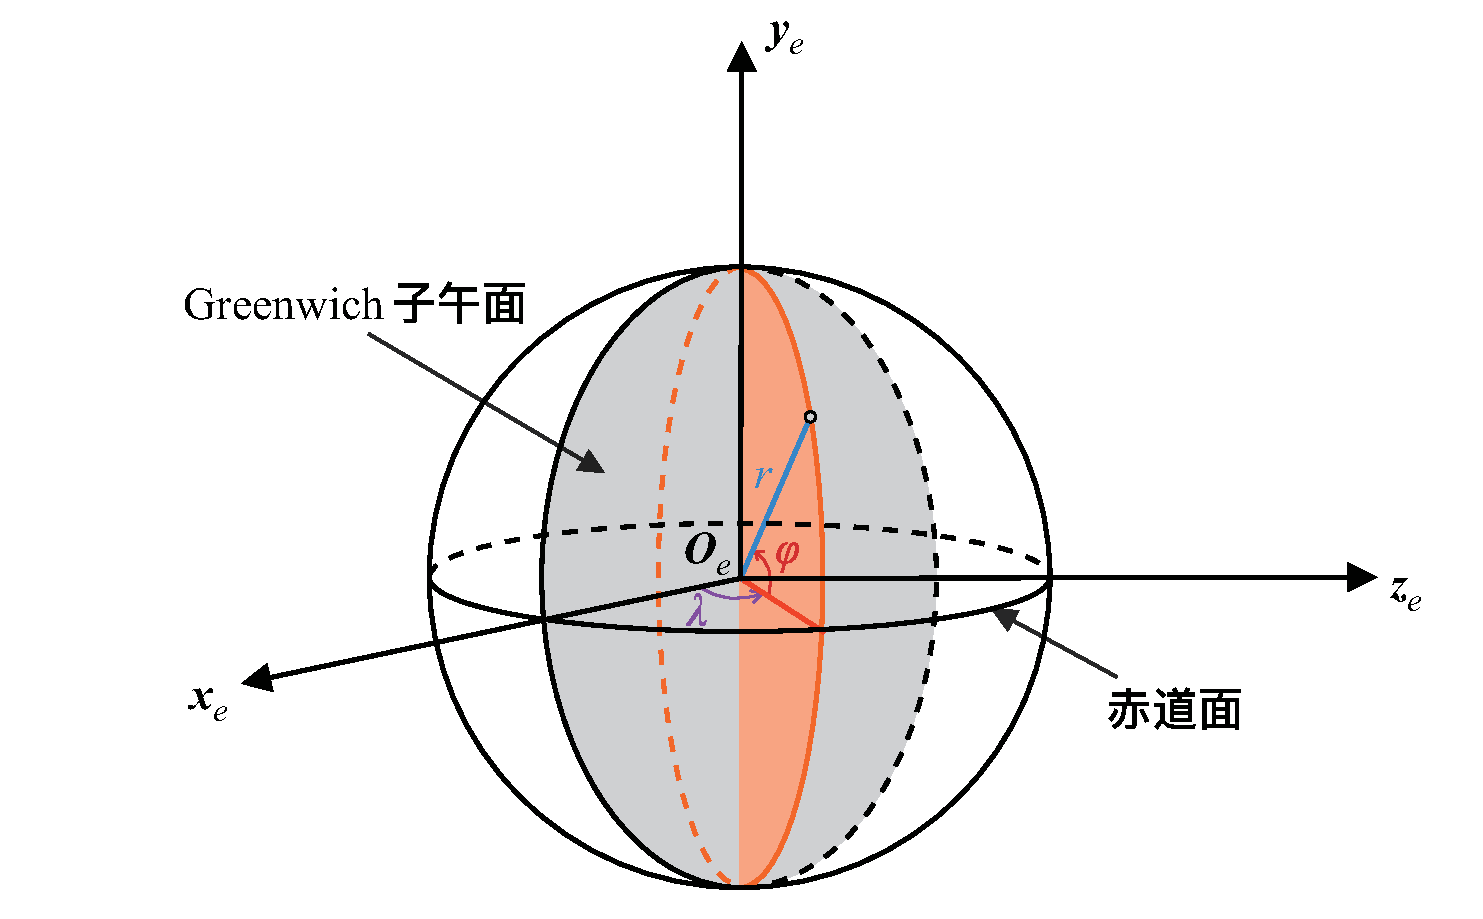
\includegraphics[width=\linewidth]{pic/地心旋转}
		\caption{地心赤道旋转坐标系}
		\label{地心旋转}
	\end{minipage}
	\begin{minipage}{0.515\linewidth}
		\centering
		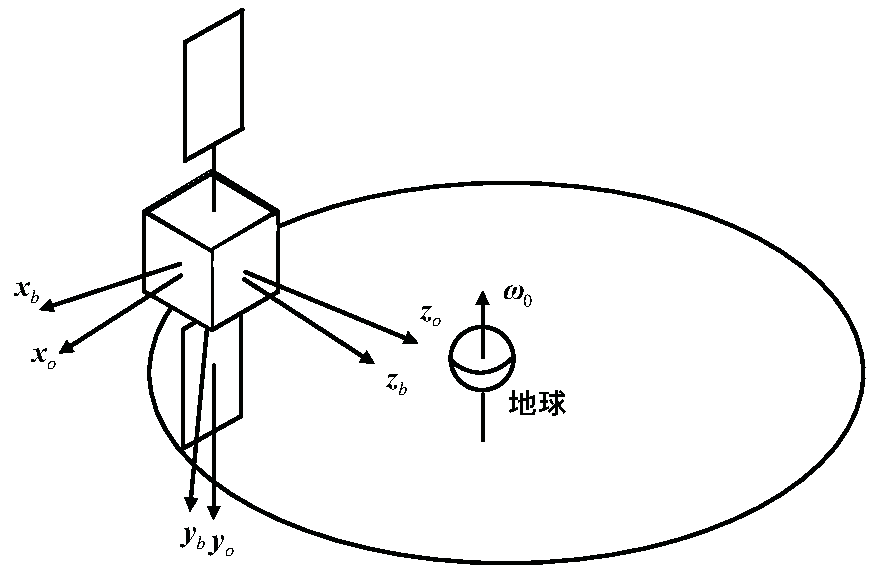
\includegraphics[width=\linewidth]{pic/轨道星体}
		\caption{轨道坐标系和星体坐标系}
		\label{轨道星体}
	\end{minipage}
\end{figure}


\subsection{轨道坐标系和星体坐标系}
\vspace*{-1em}

\defination[地心赤道坐标系]
{
	\dy[轨道坐标系]{DY}\quad 原点在飞行器质心,$z_o$轴指向地心,$x_o$轴在轨道面内与$z_o$轴垂直,指向速度方向,$y_o$轴在轨道平面法线方向,与$x_o$,$z_o$轴成右手正交坐标系。\\
	\hspace*{2.2em}\dy[星体坐标系]{XTZBX}\quad 原点在质心,$x_b$轴为滚动轴,$y_b$轴为俯仰轴,$z_b$轴为偏航轴。(对地定向航天器)
}


\section{姿态参数}
\subsection{方向余弦矩阵}
	对于坐标系原点重合的两个不同的坐标系$S_a$和$S_b$,坐标基分别为$\bm{e}_a$和$\bm{e}$
,对于矢量$\bm{u}$在两个坐标系下的分解,有
\begin{equation}
	\bm{u} = \bm{e}_b^Tu_b = \bm{e}_a^Tu_a
\end{equation}
两边同时乘以$\bm{e}_b$,得
\begin{equation*}
	\bm{e}_b \bm{e}_b^T u_b = \bm{e}_b \bm{e}_a^T u_a \quad \Rightarrow \quad u_b = \bm{e}_b\bm{e}_au_a^T
\end{equation*}
为此我们定义坐标系$S_a$变换为坐标系$S_b$的\dy[方向余弦矩阵]{FXYXJZ}为
\begin{equation}
	\bm{C}_{ba} = \bm{e}_b \bm{e}_a^T
	=
	\begin{bmatrix}
		\bm{i}_b \cdot \bm{e}_a \\
		\bm{j}_b \cdot \bm{e}_a \\
		\bm{k}_b \cdot \bm{e}_a 
	\end{bmatrix}
	=
	\begin{bmatrix}
		\bm{i}_b \cdot \bm{i}_a & \bm{i}_b \cdot \bm{j}_a & \bm{i}_b \cdot \bm{k}_a \\
		\bm{j}_b \cdot  \bm{i}_a & \bm{j}_b \cdot \bm{j}_a & \bm{j}_b \cdot \bm{k}_a \\
		\bm{k}_b \cdot  \bm{i}_a & \bm{k}_b \cdot \bm{j}_a & \bm{k}_b \cdot \bm{k}_a 
	\end{bmatrix}
	=
	\begin{bmatrix}
		C_{11} & C_{12} & C_{13} \\
		C_{21} & C_{22} & C_{23} \\
		C_{31} & C_{32} & C_{33}
	\end{bmatrix}
\end{equation}
方向余弦矩阵有以下几个特征:

\newpage

\sssection[6个约束方程]
\noa[1] 模值约束
\begin{equation}
	\begin{cases}
		\,\big|\bm{i}_b\big|^2 = C_{11}^2 + C_{12}^2 + C_{13}^2 = 1\\
		\,\big|\bm{j}_b\big|^2 = C_{21}^2 + C_{22}^2 + C_{23}^2 = 1\\
		\,\big|\bm{k}_b\big|^2 = C_{31}^2 + C_{32}^2 + C_{33}^2 = 1
	\end{cases}
\end{equation}
\proof 由于$\bm{i}_b, \bm{j}_b, \bm{k}_b$的模值为1(空间绝对),所以将它们投影到坐标系$S_a$后模值仍然为1,即
\begin{equation*}
	\begin{cases}
		\,\big|\bm{i}_b \cdot \bm{e}_a\big|^2 = \big|\bm{i}_b\big|^2 = 1\\
		\,\big|\bm{j}_b \cdot \bm{e}_a\big|^2 = \big|\bm{j}_b\big|^2 = 1\\
		\,\big|\bm{k}_b \cdot \bm{e}_a\big|^2 = \big|\bm{k}_b\big|^2 = 1\\
	\end{cases}
	\qquad \Longrightarrow \qquad 
	\begin{cases}
		\,\big|\bm{i}_b\big|^2 = C_{11}^2 + C_{12}^2 + C_{13}^2 = 1\\
		\,\big|\bm{j}_b\big|^2 = C_{21}^2 + C_{22}^2 + C_{23}^2 = 1\\
		\,\big|\bm{k}_b\big|^2 = C_{31}^2 + C_{32}^2 + C_{33}^2 = 1
	\end{cases}
\end{equation*}

\noa[2] 几何约束
\begin{equation}
	\begin{cases}
		\,\bm{i}_b \cdot \bm{j}_b = C_{11}C_{21} + C_{12}C_{22} + C_{13}C_{23} = 0 \\
		\,\bm{i}_b \cdot \bm{k}_b = C_{11}C_{31} + C_{12}C_{32} + C_{13}C_{33} = 0 \\
		\,\bm{j}_b \cdot \bm{k}_b = C_{21}C_{31} + C_{22}C_{32} + C_{23}C_{33} = 0
	\end{cases}
\end{equation}
\proof 由于$\bm{i}_b, \bm{j}_b, \bm{k}_b$两两正交(空间绝对),所以将它们投影到坐标系$S_a$后仍然满足几何关系,即
\begin{equation*}
	\begin{cases}
		\,\bm{i}_b \cdot \bm{j}_b = \big(\bm{i}_b \cdot \bm{e}_a\big) \cdot  \big(\bm{j}_b \cdot \bm{e}_a\big) = 0\\
		\,\bm{i}_b \cdot \bm{k}_b = \big(\bm{i}_b \cdot \bm{e}_a\big) \cdot \big(\bm{k}_b \cdot \bm{e}_a\big) = 0\\
		\,\bm{j}_b \cdot \bm{k}_b =\big(\bm{j}_b \cdot \bm{e}_a\big) \cdot \big(\bm{k}_b \cdot \bm{e}_a\big) = 0
	\end{cases}
	\qquad \Longrightarrow \qquad 
	\begin{cases}
		\,\bm{i}_b \cdot \bm{j}_b = C_{11}C_{21} + C_{12}C_{22} + C_{13}C_{23} = 0 \\
		\,\bm{i}_b \cdot \bm{k}_b = C_{11}C_{31} + C_{12}C_{32} + C_{13}C_{33} = 0 \\
		\,\bm{j}_b \cdot \bm{k}_b = C_{21}C_{31} + C_{22}C_{32} + C_{23}C_{33} = 0
	\end{cases}
\end{equation*}


\sssection[坐标变换矩阵是正交矩阵]

由于
\begin{equation*}
	\begin{cases}
		\,\bm{e}_b \cdot \bm{e}_b^T = \bm{e}_a \cdot \bm{e}_a^T = \bm{E}_3\\
		\,\bm{e}_b \cdot \bm{e}_b^T = \bm{C}_{ba}\bm{e}_a \cdot \big( \bm{C}_{ba} \bm{e}_a \big)^T =  \bm{C}_{ba}\bm{e}_a \cdot \bm{e}_a^T \bm{C}_{ba}^T 
	\end{cases}
	\quad \Rightarrow \quad \bm{E}_3 = \bm{C}_{ba} \cdot \big( \bm{e}_a \cdot \bm{e}_a^T \big) \cdot \bm{C}_{ba}^T =  \bm{C}_{ba} \cdot \bm{C}_{ba}^T
\end{equation*}
所以可以得到
\begin{equation}
	\bm{C}_{ba}^T = \bm{C}_{ba}^{-1}
\end{equation}
且有
\begin{equation}
	\bm{C}_{ab} = \bm{e}_a \cdot \bm{e}_b^T = \bm{e}_a \cdot \bm{e}_a^T \bm{C}_{ba}^T = \bm{C}_{ba}^{-1}
\end{equation}


\sssection[坐标变换矩阵的行列式为1]

由于














